  %# -*- coding: utf-8-unix -*-
%%==================================================
%% chapter03.tex for SJRU Master Rhesis
%% related work
%%==================================================
%\bibliographystyle{sjtu2}%[此处用于每章都生产参考文献]

% equation有编号 displaymath无编号

\theoremstyle{definition}
\newtheorem{definition}{定义}[section]

\chapter{相似轨迹查询方法实现}
\label{chap:implementation}

\section{k最佳连接}
\label{sec:k-bct}
一个轨迹数据库中存储了大量的原始车载GPS轨迹或是已经预处理过的车载GPS轨迹。这里的轨迹由一系列的地理位置点组成$\{p_{1},p_{2},p_{3},\cdots, p_{m}\}$,其中$p_{i}$ $1\leq i \leq m$代表一个由经度和维度构成的地理位置点而$m$代表轨迹中点的数目。本文所定义的k最佳连接查询(k Best-Connected Rrajectory Query)的输入由一组查询点$Q$组成。$q_{j}$ $1 \leq j \leq n$和$p_{i}$定义相同,其中n是查询点的数目。这里用户可以选择选择是否在查询中指定轨迹连接依照查询点的先后顺序,即是否选择查询有序性。若选择查询有序性,则查询点集$Q$为认为是从$q_{1}$到$q_{m}$有序点集。
\begin{displaymath}
	Q = \{q_{1},q_{2},q_{3},\cdots, q_{n}\}
\end{displaymath}

在搜索最好连接轨迹这一上下文中,相似度方程的定义需要和传统方法有所不同,在这里我们将相似度方程定义为一条轨迹连接查询点的好坏程度。因此,本文首要考虑一条轨迹到每一个查询点的距离,我们简要定义距离一个查询点$q_{i}$到一条轨迹$R=\{p_{1},p_{2},p_{3},\cdots, p_{m}\}$的距离为$D_{q}$,即

\begin{equation}
	\label{eq3-1}
	D_{q}(q_{i}, R) = \min_{p_{j} \in R} \{D_{e}(q_{i}, p_{j})\} 
\end{equation}

式\ref{eq3-1}中,$D_{e}(q_{i}, p_{j})$是指查询点$q_{i}$和轨迹点$p_{j}$之间的欧氏距离,因此通常意义上相似度距离$D_{q}$代表从查询点$q_{i}$到轨迹上任一一点距离的最短距离。当我们找到轨迹上一点$p_{j}$是离查询点$q_{i}$的最短距离点时,我们将$<q_{i},p_{j}>$作为匹配点对。在无序查询点击中,我们定义查询点集$Q$和轨迹$R$之间的相似度为$Sim(Q,R)$。

\begin{equation}
	\label{eq3-2}
	Sim(Q,R) = \sum_{i=1}^{n} \emph{e}^{-D_{q}(q_{i}, R)}
\end{equation}

式\ref{eq3-2}将每个查询点对$Sim(Q,R)$的贡献值通过自然对数去反体现,即根据自然函数的单调性,查询点离轨迹越近,则$-D_{q}(q_{i}, R)$越大,以自然对数为底取幂的值也越大,最后使得$Sim(Q,R)$的值也越大。从用户人为角度和地理语义角度上看,一条轨迹与所有的查询点被定义为相似当且仅当这条轨迹和所有的查询点都十分接近。

图\ref{fig:3-1}通过距离说明查询点和轨迹之间的匹配关系。如图\ref{fig:3-1}(a)所示,查询点$q_{1}$、$q_{2}$和$q_{3}$分别与轨迹R上的轨迹点$p_{6}$、$p_{4}$和$p_{7}$最近匹配,根据式\ref{eq3-2}可以得出,$Sim(Q,R) = \emph{e}^{-D_{q}(q_{1}, p_{6})} + \emph{e}^{-D_{q}(q_{2}, p_{4})} + \emph{e}^{-D_{q}(q_{3}, p_{7})} = \emph{e}^{-1.5}+ \emph{e}^{-0.1} + \emph{e}^{-0.1}$。

另一方面,选择查询点和轨迹之前进行有序查询时,顺序性是需要在查询过程中予以考虑。对于查询点$q_{i}$而言,最近匹配点或许并不在是距离上最近的轨迹点$p_{j}$。因此,相似度方程在此步骤中应该适当调整。我们再借用图\ref{fig:3-1}予以说明。假设以下用户场景:用户希望查询出一条以$q_{1} \rightarrow q_{2} \rightarrow q_{3}$为顺序的相似轨迹,显然图\ref{fig:3-1}(a)中的顺序并不再符合用户需求。实际的有序查询结果顺序如图\ref{fig:3-1}(b)是$p_{3} \rightarrow q_{4} \rightarrow q_{7}$。在考虑有序性的相似查询规程中,我们的目标是在保持查询有序性的同时追求每一对匹配点对相似度的最大贡献值,即从图\ref{fig:3-1}(b)可以看出$<q_{1},p_{3}>, <q_{2},p_{4}>, <q_{3},p_{7}>$这样的三对匹配点是所有有序匹配对中使得相似度最大的情况。

\begin{figure}[!htp]
  \centering
  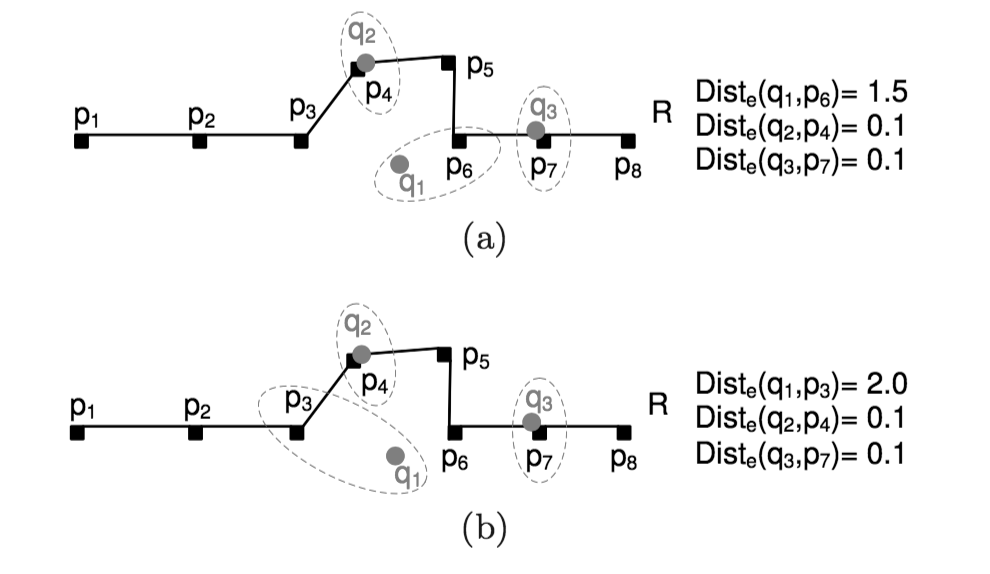
\includegraphics[width=0.7\textwidth]{chapter03/similarity.png}
  \bicaption[fig:3-1]{这里将出现在插图索引中}{查询点与轨迹之间的匹配}{Fig}{Match between query points and trajectory}
\end{figure}

有序查询的相似性计算和无序查询也有区别。给定一组有序的查询点$Q_{o} = \{q_{o1},q_{o2},q_{o3},\cdots, q_{on}\}$和一条已有轨迹$R$,我们通过递归思想为有序查询重新定义相似度方程为$Sim_{o}(Q,R)$,式\ref{eq3-3}。其中$Head(x)$函数代表$x$中的第一个点,例如$Head(Q)$是查询点$q_{1}$;同时$Rest(x)$表示$x$去掉x第一个点之后剩余的部分,例如$Rest(Q)$代表\{$q_{2},q_{3},\cdots, q_{n}$\}。在式\ref{eq3-3}中,通过递归的想法,本文将对$Sim_{o}(Q,R)$的求最大值问题分为对两个子问题的求解,即分别计算$Sim_{o}(Rest(Q),R)$和$Sim_{o}(Q,Rest(R))$的最大值问题。当$Head(Q)$和$Head(R)$的两个轨迹点匹配的时候,我们可以将$e^{-D_{e}(Head(Q), Head(R))}$提前计算并加入当后面计算的$Sim_{o}(Rest(Q),R)$之中。在这种情况下,$Head(R)$需要为下一轮的比较计算继续保留,因为对于$Rest(Q)$中的查询点来说,$Head(R)$依旧有可能成为最佳匹配点。而当当$Head(Q)$和$Head(R)$不匹配的时候时我们则跳过$Head(R)$计算$Sim_{o}(Q,Rest(R))$。这种求解思路类似于动态规划的思路,这也为我们再后面优化过程中通过动态规划的来解决这一问题提供了参考。式\ref{eq3-3}结合了动态时间规整(DTW)利用重复点和最长公共子序列(LCSS)省略不匹配点的优点来计算相似度方程。

\begin{equation} 
\label{eq3-3} 
Sim_{o}(Q,R)= max \left\{  
	\begin{array}{lr}  
    e^{-D_{e}(Head(Q), Head(R))} + Sim_{o}(Rest(Q),R) & \\
    Sim_{o}(Q,Rest(R)) &  
    \end{array}  
\right.  
\end{equation}  

根据相似度方程,本文可以对k最佳连接查询有以下定义3.1.1.:

%\begin{thm}[k最佳连接]
%	给定一组轨迹集合 $T = {R_{1}, R_{2}, R_{3} \cdots, R_{n}}$、一组查询点$Q = {q_{1},q_{2},q_{3},\cdots, q_{n}}$和对应的相似度方程$Sim$,k最佳连接查询则可以从轨迹集合$T$中找到k条轨迹$T'$,满足式\ref{eq3-4}:
%	\begin{equation}
%		\label{eq3-4}
%		Sim(Q,R_{i})_{R_{i} \in T'} \geq Sim(Q,R_{j})_{R_{j} \in T-T'}
%	\end{equation}
%	其中$Sim$根据用户定义选择是否考虑有序性。
%\end{thm}

\theoremstyle{definition}
\begin{definition}
	给定一组轨迹集合 $T = {R_{1}, R_{2}, R_{3} \cdots, R_{n}}$、一组查询点$Q = {q_{1},q_{2},q_{3},\cdots, q_{n}}$和对应的相似度方程$Sim$,k最佳连接查询则可以从轨迹集合$T$中找到k条轨迹$T'$,满足式\ref{eq3-4}。其中$Sim$根据用户定义选择是否考虑有序性。:
	\begin{equation}
		\label{eq3-4}
		Sim(Q,R_{i})_{R_{i} \in T'} \geq Sim(Q,R_{j})_{R_{j} \in T-T'}
	\end{equation}
\end{definition}

\section{相似轨迹查询处理过程}
\label{sec:query processing}
完成上述k最佳连接查询,我们首先需要明确我们查询输入的优势在于我们输入的查询点相对于传统的相似轨迹查询方法要小。这是我们能够合理且有效运用空间索引分别对每一个查询点应用近邻查询,并合并查询结果生成k最佳连接结果的基本前提。这一方法的搜索复杂度相对于查询点集来说相对恒定。因此,当得出一条轨迹对于查询点集的最近轨迹点便为我们计算该条轨迹与查询点集相似度的上下界提供可能。本文中使用R树索引并搜索近邻的轨迹点,当我们找到关于某个查询点$q$的最近轨迹点$p$,那么包含$p$轨迹点的轨迹一定是离该查询点$q$最近的一条轨迹。本文的相似轨迹查询方法利用R树数据结构,通过简单的k最近邻算法并在其基础上进行有效深度拓展和具体实践优化实现k最佳连接查询以实现相似轨迹查询。表\ref{tab-notations}提供了本文需要的基本符号及其注释。
\\

\begin{table}[!htpb]

  	\centering
		\begin{tabular}{ |p{3cm}||p{9cm}|  }
		\hline
		符号标记 & 符号注释 \\
		\hline
		$N$ & 一条轨迹的轨迹点总数目 \\
		\hline
		$m$ & 一组查询点总数目 \\
		\hline
		$D_{e}(q_{i},p_{j})$ & 点$q_{i}$和点$p_{j}$之间的欧氏距离 \\
		\hline
		$D_{e}(q_{i},p_{j})$ & 点$q_{i}$和点$p_{j}$之间的欧氏距离 \\
		\hline
		$D_{q}(q_{i},R)$ & 点$q_{i}$和轨迹$R$之间的最短距离 \\
		\hline
		$C$ & 轨迹备选集 \\
		\hline
		$\epsilon$ & TBD\\
		\hline
		$r$ & $\lambda$-NeareatNeighbor搜索半径\\
		\hline
		$\rho$ & 轨迹点密度\\
		\hline
		$\xi$ & 查询点$q_{i}$对相似度上界贡献度\\
		\hline
		$\mu,\upsilon$ & 优化搜索权值\\
		\hline
		\end{tabular}
	\bicaption[tab-notations]{出现在表目录的标题}{本文符号列表及其对应注释}{Table}{A list of notations and explanations}
\end{table}

\subsection{增长型k最近邻查询方法}
\label{subsec:iknn}
将预处理的轨迹点存储在R树之中后,我们可以有效地通过k最近邻搜索方法来找到离某一查询点$q$最近的一条轨迹。假设现有一组查询点$Q = \{q_{1},q_{2},\cdots, q_{m}\}$,进行无序的相似轨迹查询。我们首先对这一组查询点中的每一个查询点进行$\lambda NN$查询并得到结果如下:

\begin{align*}
\lambda NN(q_{1}) &= \{p_{1}^{1}, p_{1}^{2}, p_{1}^{3}, \cdots, p_{1}^{\lambda}\}\\ 
\lambda NN(q_{2}) &= \{p_{2}^{1}, p_{2}^{2}, p_{2}^{3}, \cdots, p_{2}^{\lambda}\}\\ 
\cdots\\
\lambda NN(q_{m}) &= \{p_{m}^{1}, p_{m}^{2}, p_{m}^{3}, \cdots, p_{m}^{\lambda}\}
\end{align*}

通过每个查询点根据$\lambda NN$算法生成的结果,我们根据结果中的点生成我们的轨迹备选集。包含$\lambda NN(q_{i})$中至少一个轨迹点的轨迹被加入到轨迹备选子集$C_{i}$中用于之后生成k最佳连接结果。在这一步我们需要保证轨迹备选子集$C_{i}$的基数应该小于等于$\lambda$,因为多个属于$\lambda NN(q_{i})$的轨迹点有可能属于同一条轨迹。之后我们合并所有由$\lambda NN(q_{i})$查询结果得出的轨迹备选子集以获取一个包含$f$条轨迹的轨迹备选集$C$

\begin{equation} 
 C = \bigcup_{i=1}^{m} C_{i} = \{R_{1}, R_{2}, \cdots, R_{f}\} \nonumber
\end{equation}  

对于轨迹备选集$C$中的每一条轨迹$R_{x} (1 \leq x \leq f)$而言,$R_{x}$必须包含至少一个离对应查询点距离在固定范围内的轨迹点。即假使$R_{x}$属于某一轨迹备选子集$C_{i}$($C_{i}$为轨迹备选集$C$的子集),那么$\lambda NN(q_{i})$中的应该包含轨迹$R_{x}$上的一点且$q_{i}$到轨迹$R_{x}$的最短距离是已经计算过的。由于轨迹$R_{x}$和查询点$q_{i}$至少有一组已知的匹配点,则我们可以通过已知匹配点来计算出轨迹备选集中轨迹与查询点集相似度的下界,我们定义为$LB$(lower bound)。

\begin{equation}
	\label{eq3-5}
	LB(R_{x}) = \sum_{1\leq i\leq m \wedge R_{x}\in C_{i}}\bigg( \max_{1\leq j\leq \lambda \wedge p_{i}^{j}\in R_{x}}e^{-D_{e}(q_{i}, p_{i}^{j})}\bigg)
\end{equation}


在计算下界的时候,我们考虑的查询点集为$Q_{matched}$ = \{$q_{i} | 1\leq i\leq m \wedge R_{x} \in C_{i}$\},对于$Q_{matched}$中的查询点来说,他们和轨迹$R_{x}$上的某一个轨迹点在进行k最近邻查询中被计算作为匹配点,即对于查询点$q_{i} \in Q_{matched}$,我们可以找到轨迹上的某一点$p_{i}^{j}$满足$e^{-D_{e}(q_{i}, p_{i}^{j})}$达到最大值,因为在欧氏距离上$q_{i}$与$p_{i}^{j}$最为接近,根据这一点我们可以将式\ref{eq3-5}中的$\max_{1\leq j\leq \lambda \wedge p_{i}^{j}\in R_{x}}e^{-D_{e}(q_{i}, p_{i}^{j})}$等价写成$e_{-D_{q}(q_{i}, R_{x})}$,得出式\ref{eq3-6}

\begin{equation}
	\label{eq3-6}
	LB(R_{x}) = \sum_{1\leq i\leq m \wedge R_{x}\in C_{i}}e^{-D_{q}(q_{i}, R_{x})}
\end{equation} 

显然这个相似度下界值不会大于$\sum_{i=1}^{m} e^{-D_{q}(q_{i}, R(x))}$,因为在计算相似度下界的时候值考虑了与在轨迹$R_{x}$上与某些查询点匹配轨迹点。另一方面,加入轨迹$R_{x}$不属于某个备选轨迹子集$C_{i}$,则轨迹$R_{x}$上任意轨迹点都不会存在于由查询点$q_{i}$得到的k最近邻查询结果$\lambda NN$中。这说明由式\ref{eq3-5}或\ref{eq3-6}定义的相似度下界计算对于式\ref{eq3-2}是成立的。

对于在不属于轨迹备选集$C$中的轨迹($R_{ns} \notin C$),这些轨迹并没有在查询点集进行k最近邻查询中被扫描,他们到查询点$q_{i}$的距离将会小于$p_{i}^{\lambda}$到查询点$q_{i}$的最短距离,即$D_{e}(q_{i}, p_{i}^{\lambda})$。这一发现能让我们计算出所有不属于轨迹备选集的轨迹$R_{ns}$对于查询点集的相似度的上界,我们定义为定义为$UB_{ns}$(upper bound)。

\begin{equation}
	\label{eq3-7}
	UB_{ns} = \sum_{i=1}^{m}e^{-D_{e}(q_{i}, p_{i}^{\lambda})}
\end{equation}

当我们在进行有关空间意义上的数据搜索的时候,剪枝是保证搜索效率的重要手段。相似度的上下界让我们可以设计出针对k最佳连接的剪枝算法以限制搜索空间,提高搜索效率,避免了对整个轨迹数据集或者对不满足条件的轨迹进行多余操作。根据相似度的上下界我们提出下述定理:
\\

\begin{thm}[相似度上下界]
	\label{thm3-1}
	假设对于相似轨迹插叙的k最佳连接算法没有有序性限制,我们可以在对查询点集进行一轮k最近邻查询(k=$\lambda$)之后的轨迹备选集C中,选取一个包含k条轨迹的一个轨迹子集$C'$。当$\min_{R_{x}\in C'}{LB(R_{x})}\geq UB_{us}$这一条件满足时,我们可以从轨迹备选集$C$中获得k条最佳连接轨迹,即k条与查询点集最相似的轨迹。
	\begin{proof}
	首先对于轨迹子集$C'$中的某一条轨迹$R_{a}$($R_{a} \in C'$)而言,轨迹$R_{a}$满足$Sim(Q,R_{a}) \geq LB(R_{a})$。与此同事,对于轨迹备选集$C$之外的轨迹$R_{b}$($R_{b} \notin C$),轨迹$R_{b}$满足$UB_{ns} \geq Sim(Q,R_{b})$。当上述定理成立时,即$\min_{R_{a}\in C'}{LB(R_{a})}\geq UB_{ns}$,我们可以推断出$\forall R_{a}\forall R_{b} \big( R_{a} \in C' \wedge R_{b} \notin C \big)$,$Sim(Q,R_{a}) \geq Sim(Q,R_{b})$成立。这也证明了对于查询点集$Q$得到的k最佳连接的结果轨迹在这个时候应该全部在轨迹备选集$C$中。
	\end{proof}
\end{thm}

需要注意的是定理\ref{thm3-1}中的轨迹子集$C'$不一定全是k最佳连接轨迹的结果,我们只能保证k最佳连接的轨迹在轨迹备选集$C$中。而定理\ref{thm3-1}是我们在进行k最近邻查询而找到k最佳连接轨迹的保证条件。

在搜索过程中我们需要解决一个关键问题就是$\lambda$的取值问题,$\lambda$值的大小决定了我们的k最佳连接轨迹,即k最相似轨迹是否存在于轨迹备选集$C$中。在定理\ref{thm3-1}中我们的轨迹备选集$C$的基数大小从在很大程度上取决于我们设定的查询$\lambda$值的大小。假如$\lambda$的值我们取的较大,则k最佳连接轨迹基本包含于轨迹备选集$C$内,但这样会造成搜索空间过大的问题。另一方面,$\lambda$过小会使得轨迹备选集$C$不完全包含k最佳连接轨迹,导致搜索的不准确性和错误性。为了解决$\lambda$的取值问题,我们尝试通过动态调整$\lambda$值的方法来一步步满足查询结果,这是我们提出\emph{增长型k最近邻查询算法}的基本思想。增长性k最近邻查询算法是基于备选和筛选模式获取备轨迹的高效算法,其大致思想是在算法开始对每一个查询点初步进行k最近邻查询($k=\lambda$,最初$\lambda$可以是任一正整数值)。查询结果如果不满足定理\ref{thm3-1}条件,我们再在$\lambda$值上进行动态增加$\Delta\lambda$,将查询范围从$\lambda$增加到$(\lambda+\Delta\lambda)$,然后我们进行$(\lambda+\Delta\lambda)$最近邻查询。持续这一过程直到我们找到满足定理\ref{thm3-1}条件的$\lambda$值。实现过程伪代码为算法\ref{algo:iknn}所示。

%\begin{algorithm}
\begin{algorithm}[H] % 强制定位
\caption{增长型k最近邻查询算法}
\label{algo:iknn}
\begin{algorithmic}[1] %每行显示行号
\Require 相似轨迹查询数目$k$, 查询点集$Q$ % 输入
\Ensure k条最相似轨迹$k$-$Trajs$ % 输出

\State Candidate Set $C$; //初始化轨迹备选集$C$
\State Initialise Upper bound of Similarity $UB_{ns}$; //初始化轨迹相似度上界
\State Initialise Lower bounds $LB[]$, $k-LB[]$; //初始化两个有关相似度下界的数组
\State $\lambda \gets k$ //将k值初始赋值给$\lambda$
\While {true}
	\For{each $q_{i} \in Q$ that $1\leq i\leq m$}
		\State $C_{i}\gets$ trajectories that contains the points in $\lambda$-$NN(q_{i})$;
	\EndFor
	\State $C \gets\bigcup_{i=1}^{m}C_{i}$; //合并轨迹备选子集以生成轨迹备选集C
	\If {$|C| \geq k$}
		\State compute $LB[]$ for all trajectories in $C$; //计算轨迹备选集C中的所有轨迹相似度下界
		\State compute $UB_{ns}$; //计算相似度上界
		\State $k$-$LB[]\gets$ $LB[]$.heapKtop(); //选取相似度下界k个最大值和其对应的轨迹
		\If {$k$-$LB[].min\geq UB_{ns}$} //满足定理\ref{thm3-1}
			\State $k$-$Trajs\gets refine(C)$ //轨迹筛选方法
			\State \textbf{return} $k$-$Trajs$ 
		\EndIf
		 
	\EndIf
\EndWhile
	

\end{algorithmic}
\end{algorithm}

